\subsection{System design}
\label{sec:aSTEPCommunication.tex}
This section will describe the communication between the \gls{rs} system and the \gls{astep} system, and how features from the \gls{astep} API are used to achieve the required functionality.
The \gls{rs} system continues the three part design, as explained in \ref{sec:s2systemdesign}, but has to adjust to the \gls{astep} progression and changes.

Since the \gls{astep} API is a REST API, all API calls are done through HTTP requests.
The \gls{astep} system provides an assortment of API functions, but the \gls{rs} system will only be using a subset of the features: Routes and Users, excluding categories such as indoor LBS.
The API functions are utilized to send recorded routes to \gls{astep}, and to create new \gls{astep} users.
As there are restrictions regarding user information sharing internal in \gls{astep}, it is necessary to allow \gls{rs} to access data from the \gls{astep} server external.
An overview of the API functionality as of sprint 3 can be found in Appendix \ref{ch:appAlabel}. 

\subsection{User management}\label{subsec:usermanagement}
%why UM
User management must be performed for the \gls{rs} system to utilize the route-matching algorithm because the algorithm requires access to the routes and locations based on the different users.

% how-to
There are two ways of resolving user data sharing using the \gls{astep} API.
The first solution is to create a group for all the \gls{rs} users.
The second is to create one administrating \gls{rs} user that has an access edge to every \gls{rs} user in \gls{astep} system.
The alternatives are elaborated in the following paragraphs.

\textbf{Groups}\\ 
Groups in the \gls{astep} system exist to allow users to gain access to each others data.
This could be utilized by making a \gls{rs} group in which all \gls{rs} users are included.
An issue with this solution is that all users have granted all other users access to their own location data. 
The solution allows a malicious programmer to create a program that either copies or edits the locations of all users of the \gls{rs} app.
The intruder would only need a registered \gls{rs} user and would thereby be included in the group.

\begin{figure}[h]
	\centering
	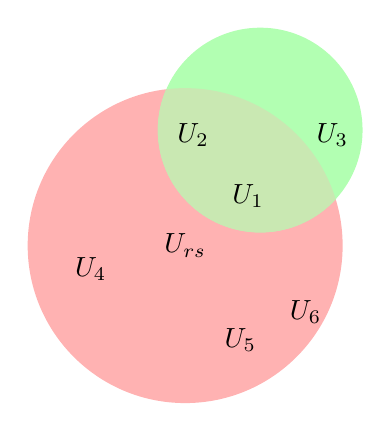
\begin{tikzpicture}
		\path[fill=red!30] (0:0cm) circle (2cm);
		\path[fill=green!30] (57:1.75cm) circle (1.3cm);
	
		\begin{scope}
			\clip(57:1.75cm) circle (1.3cm);
			\path[fill=red!30!green!30] (0:0cm) circle (2cm);
		\end{scope}
		
		\node at (0,	0) 		{$U_{\gls{rs}}$};
		\node at (0.8,	0.63) 	{$U_1$};
		\node at (0.1,	1.4)	{$U_2$};
		\node at (1.87,	1.4) 	{$U_3$};
		\node at (-1.2,	-0.3)	{$U_4$};
		\node at (0.7,	-1.2) 	{$U_5$};
		\node at (1.53, -0.84) 	{$U_6$};
	\end{tikzpicture}
	\label{fig:astepgroup}
	\caption{How \gls{rs} would use groups. In the red group all users in that group can see all data from other users in the same group.}
\end{figure}

\textbf{Edges}\\ 
Edges work in a similar way to groups, but only allowing access from one user to another.
This can be accomplished by establishing communication using the same method as with the groups and creating a \gls{rs} user and instantiate an edge from the \gls{rs} user to every other user in the \gls{rs} system, illustrated in Figure \ref{fig:astepedge}.
This way, only when the \gls{rs} system uses its own user the remaining user data can be accessed.

\begin{figure}[h]
	\centering
	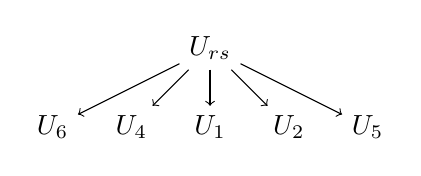
\begin{tikzpicture}
		
		\node (r) {$U_{\gls{rs}}$};
		\node[below of=r] (1) {$U_1$};
		\node[right of=1](2) {$U_2$};
		\node[left of=1] (4) {$U_4$};
		\node[right of=2] (5) {$U_5$};
		\node[left of=4] (6) {$U_6$};
		
		\draw[->] (r) -- (1);
		\draw[->] (r) -- (2);
		\draw[->] (r) -- (4);
		\draw[->] (r) -- (5);
		\draw[->] (r) -- (6);
		
		%\draw[->] (1) -- (4);
	\end{tikzpicture}
	\caption{How \gls{rs} would work with edges.}
	\label{fig:astepedge}
\end{figure}

The edges method allows edges to provide the same benefits as groups for this use case while disabling the security flaw mentioned above.
Therefore, the edges method is selected as the user management design pattern.

\textbf{Creating users}\\
In sprint 2 it was also decided to create users through the \gls{rs} server, this has been changed to simplify the implementation and reduce design complexity.

When a user registers in the \gls{rs} app, the app will issue an API call directly to the \gls{astep} API, instead of performing the operation through the \gls{rs} server. 
The username and additional information, such as phone number and full name, will still be transferred to the \gls{rs} server to enable contact information sharing with other \gls{rs} users.